\section{プログラミングに対する興味喚起を目的としたプログラミングゲームの開発}
本項では,プログラミング初学者の興味喚起を目的としたプログラミングゲームのプロトタイプについて紹介し,設計指針に基づくデザインの詳細や行った評価実験と見つかった課題,実験に関する考察について議論する.

\subsection{研究背景}
プログラミングの重要性が高まり,プログラミング学習を始める人は増えているが,その中で挫折する者も多い.写経型学習では楽しさを感じにくく,またプログラミングの楽しさを感じるためには,ある程度プログラミングに習熟することが必要であることがその要因の1つであると考えられる.

プログラミングにおける難解な部分を隠蔽・抽象化することで,初学者でもプログラミングの楽しさを実感できることを目指したシステムはいくつかある.ScratchやViscuitなどのVPLがその代表的な例である.しかしこれらは小・中学生など若い世代をターゲットとして作成されているため,高校生や大学生,あるいはそれ以上の年齢の層に対して,十分な興味喚起ができているとは言えない.またこれらは初学者向けにデザインされたVPLのため,PythonやC言語といった実践的なTPLとの乖離が大きいという問題もある.

本項で述べる研究では,実践的なTPLによる初学者への興味喚起を行うため,リアルタイムな対戦型プログラミングゲームを開発した.このゲームではリアルタイムにエージェントのアルゴリズムをプログラミングし,戦わせる.この対戦型のプログラミングゲームを習熟したプログラマ同士にプレイさせ,対戦させる.これを初学者に観戦させることにより,プログラミング言語の基礎的な文法を理解しつつ,習熟したプログラマへの憧れを創出し,プログラミングへのモチベーションを向上させることを目指した.習熟したプログラマのプログラミングの様子を観察することで,プログラミングの手順・デバッグの手法を学ぶこともできると考えられる.またゲームをターン性にしたことで,アルゴリズムを考え,実装し,実行,改善するというプロセスを見て学ぶことができると思われる.


\subsection{関連研究・関連システム}

\subsubsection{プログラミングを用いたエンタテインメントシステム}
プログラミングとエンタテインメントを掛け合わせたコンテンツはいくつか存在する.TopCoder\cite{topcoder}などの競技プログラミング,コードゴルフ\cite{codegolf}やSECCON\cite{seccon}などのハッキングコンテストが有名であり,これらはプログラマの間でも根強い人気がある.またプログラミングゲームとしてはRobocode\cite{robocode}が有名である.しかしこれらはある程度プログラミングに習熟したプログラマ向けのコンテンツであり,利用にはプログラミングスキルだけでなく数学やセキュリティ,コンピュータサイエンス等の知識を要するためプログラミング初学者が参加するにはハードルが高い.

\subsubsection{初学者向けプログラミング学習支援システム}
初学者向けプログラミング学習支援システムは数多く存在する.Scratch\cite{scratch},Viscuit\cite{viscuit}などはその代表的な例であり,低年齢層をターゲットにした設計でブロックや絵を並べることでプログラミングでき,初学者にプログラミングの楽しさを伝えるためにデザインされている.塚本らの研究では,テキストベースのプログラミング言語による小学校でのプログラミング教育の可能性を示唆しているが,テキストベースのプログラミング言語とビジュアルプログラミング言語を用いた小学生向けの授業を比較し,ビジュアルプログラミング言語を用いた場合の方がモチベーションを向上させることができたと述べている.\cite{tpl,tsukamoto}またドリトル\cite{dolittle}は中学校・高等学校での教育目的に使える環境を目指し,テキストベースでプログラミングさせつつも柔軟かつ小さい言語仕様により,初学者にプログラミングの楽しさを伝えることを目指している.しかしこれらは対象がやや若年層向けであり,プログラマに対する憧れを創出し,プログラミングへのモチベーションを高めるという本研究のアプローチとは異なる.

\subsubsection{プログラミングゲームを用いた研究}
プログラミングゲームはいくつか存在するが,その中でも有名なのがRobocodeである.これはJavaでロボットを制御するプログラムを記述し戦わせるゲームであり,JuがRobocodeコミュニティを対象に行った調査では,ユーザの多くがRobocodeによりプログラミングスキルが向上したと回答し,Robocodeの楽しい点としてアルゴリズムを見つけることとアーキテクチャのデザインが挙げられていた\cite{long}.

またプログラミングゲームを盛り込むことでプログラミング学習を促進しようとした研究は多くある.Shiらはプログラミングゲームを用いてプログラミング初学者の問題解決能力を向上させるためのシステムを作成している\cite{joshua}.Morenoらはボクシング型の競争ゲームを用いてプログラミングスキルの向上を図っている\cite{julian}.水口の研究ではプログラミングの講義における成績評価にロボットバトルシミュレーション型のプログラミングゲームを活用している\cite{minakuchi}.なお増谷らの開発したVLogic\cite{mashitani}ではVR空間上にブロックベースのプログラミングゲームを実装することで手足を使ってプログラミングを体験することができ,プログラミングに対する興味喚起を行っている.これらはプログラミングの習熟度が高くなくても使用できるが,従来のプログラミングゲーム同様静的なゲーム展開であり,プログラマ同士のリアルタイムな駆け引きやアドリブといった観戦を楽しむ設計は成されていない.


\subsection{設計指針}

提案システムの実装にあたり,初学者の興味関心を高めるために3つの設計指針を設けた.

\begin{enumerate}
  \item {\bf 駆け引き・アドリブを取り入れる}

  多くの人は野球やサッカー,ラグビーなどのスポーツや将棋,麻雀などのテーブルゲーム,昨今ではストリートファイターに代表されるe-sportsなどの競技を,自分がプレイヤでなくとも観戦することを好む.これらの競技の試合は,研磨された戦法の型がありつつも,プレイヤ同士のリアルタイムな駆け引きやアドリブを伴って進行する予測不可能性が魅力の1つであり,プレイするだけでなく観戦するという行為によって古くから親しまれてきた.本項の提案システムにおいてもこのリアルタイムな駆け引き・アドリブの要素を生かし,ゲームを観戦して楽しめるようデザインし,初学者のモチベーションを高めることを目指す.

  
  \item {\bf 観戦して楽しめる}

	初学者にとってプログラミング学習をする際に環境構築や普段使用しない独自ソフトウェアのインストールは手間がかかり,学習のモチベーションを下げかねない.今回は提案システムをJavaScriptによって制御可能なWebアプリケーションとして実装し,初学者が実際にプログラミングを行わずともプログラミングしている様子を観戦するだけで利用できるように設計した.

	\item {\bf プログラミングに対する憧れを創出する}

  提案システムでは習熟したプログラマ同士のスキルを対戦に反映させることで,習熟したプログラマとその洗練されたプログラムに対する憧れを創出し,システムの利用を促すとともにプログラミングのモチベーションを向上させることを目指した.

\end{enumerate}

\subsection{提案システム}

本研究で提案するシステムでは,プログラミング初学者の興味喚起をするためにいくつかの工夫を施した.今回実装したシステムは,プログラマ同士がリアルタイムにプログラミングを行うことでキャラクタを制御し,対戦するという対人形式のプログラミングゲームである.この対戦の様子を初学者に観戦させることで,初学者のプログラミングに対する興味を高める.プログラミングゲームとして実装した理由としては,キャラクタがプログラムによって動作するというゲームの視覚的な出力が,初学者にとってプログラムの出力を理解する助けになると考えたためである.ゲームジャンルとしては,シューティングゲームの体裁をとった.これはシューティングゲームが「敵の攻撃を避けて,敵を攻撃する」というプリミティブなゲームシステムであり,見ていて展開を理解しやすいと考えたためである.

ゲームUIはLivecodeLab\cite{livecodelab}やHydra\cite{hydra}などのビジュアルライブコーディング環境を踏襲し,ゲーム画面上にエディタを重畳することで,プログラムとその出力の双方を同時に見ることが可能なように設計した.またゲーム3つのフェイズに分かれており,以下で各フェイズについて説明する.大まかなフェイズ遷移の様子を図\ref{phase}に示す.

なお2人のプレイヤが対戦する「vsPlayer」モードと1人のプレイヤがCPUと対戦する「vsComputer」モードを実装した.

\begin{figure}[!b]
  \begin{center}
    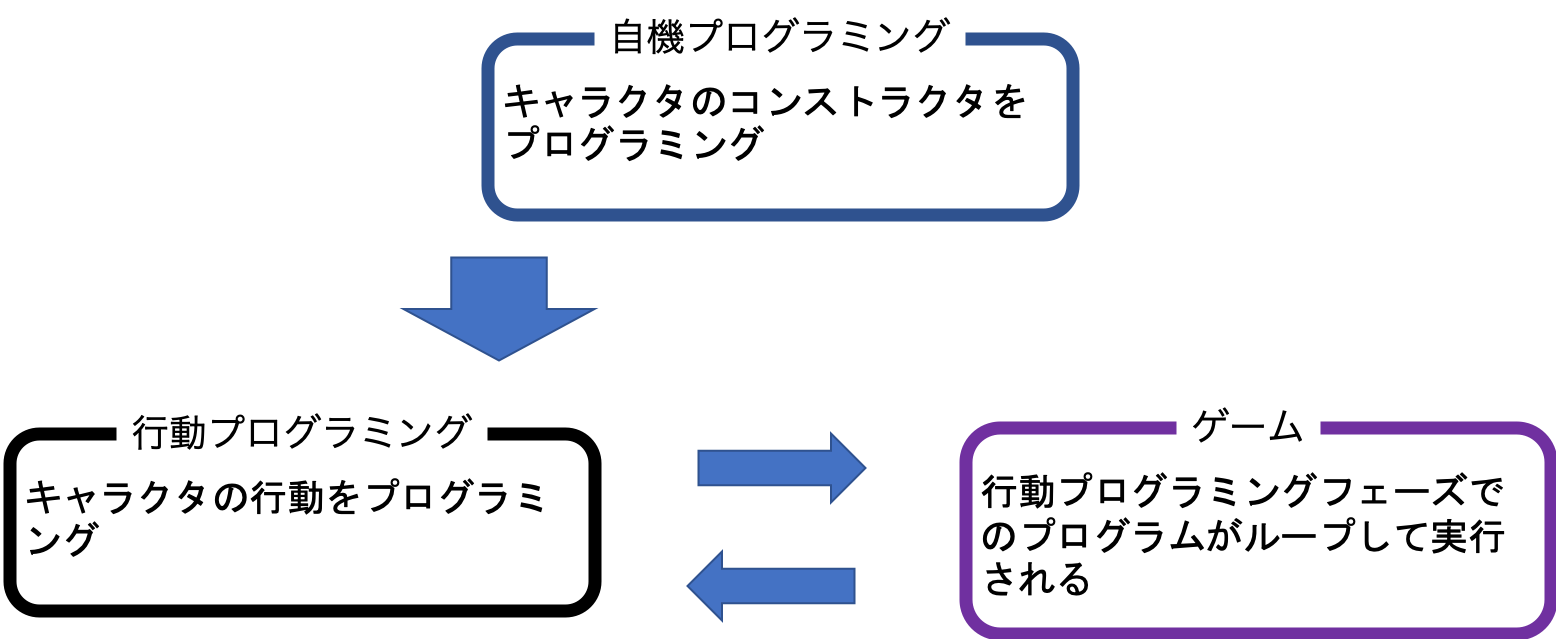
\includegraphics[width=1.0\linewidth]{image/phase.eps}
  \end{center}
    \vspace{-8mm} 
  \caption{フェイズ遷移図}
  \label{phase}
\end{figure}

\subsubsection{自機プログラミングフェイズ}
プレイヤが「vsPlayer」モードを選んで相手プレイヤとマッチングする,または「vsComputer」モードを選ぶとこのフェイズに移行する.プレイヤには1か2の番号が振られ,番号に応じて画面の背景色や制御するキャラクタの番号が異なる.このフェイズの様子を図\ref{characterProgramming}に示す.

\begin{figure}[!ht]
  \begin{center}
    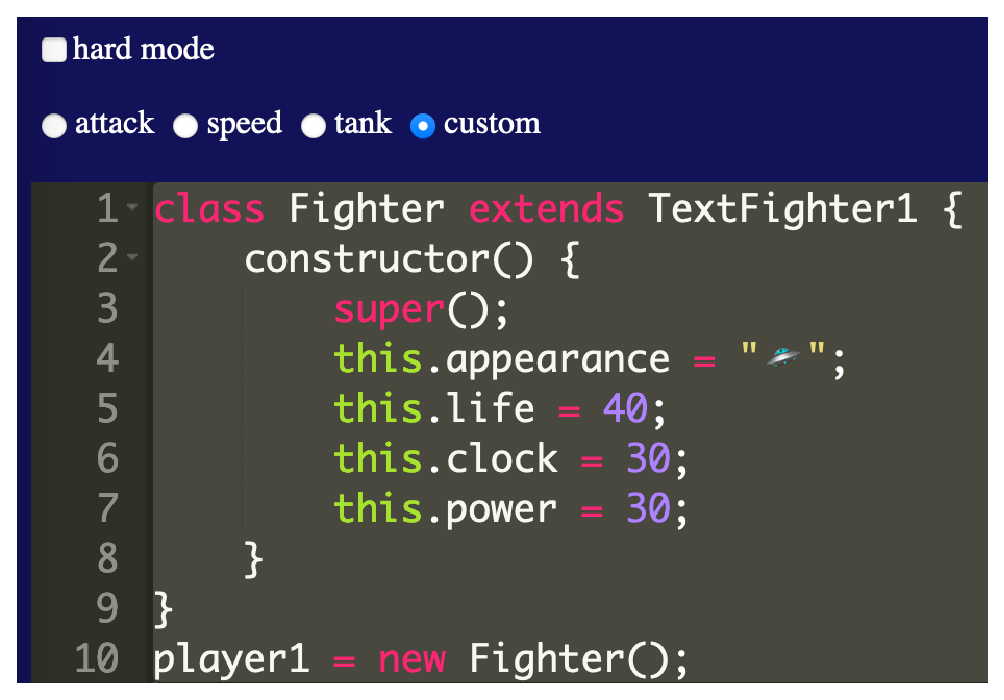
\includegraphics[width=0.8\linewidth]{image/characterProgramming.eps}
  \end{center}
    \vspace{-8mm} 
  \caption{自機プログラミングフェイズの様子}
  \label{characterProgramming}
\end{figure}

ここでは予めエディタにプレイヤが操作するキャラクタのコンストラクタが記述されており,プレイヤはパラメータを書き換えることができる.具体的なパラメータにはappearance,life,clock,powerがある.appearanceはキャラクタの外見であり,文字列を指定できるため,絵文字などを使ってプレイヤの好きな見た目を選ぶことが可能である.lifeはキャラクタの体力であり,いわゆるHP(ヒットポイント)を表している.非負の整数を指定でき,この値が0以下になるとプレイヤはゲームに敗北する.clockはキャラクタが行動できる回数の多さを表しており,非負の整数を指定できる.プレイヤは後述する行動プログラミングフェイズにおいて自分のキャラクタを制御するプログラムを記述し対戦するが,その際に記述したプログラムは10秒間ループして実行される.このループのインターバルを決めるのがclockであり,値が大きいほどインターバルは短くなる.powerはキャラクタの攻撃力を表しており,これも非負の整数を指定できる.この値が大きいほど,自分が操作するキャラクタの攻撃が相手キャラクタに命中した際に削るlifeの値が大きくなる.双方のプレイヤが各パラメータを記述し終わると次の行動プログラミングフェイズに移行する.



\subsubsection{行動プログラミングフェイズ}
このフェイズに進むと,自機プログラミングフェイズで記述したコンストラクタを元に両プレイヤが操作するキャラクタのインスタンスが作成され,ゲーム画面が表示される.このフェイズの様子を図\ref{actionProgramming}に示す.両プレイヤはプログラムをエディタに記述し,作成したキャラクタを操作する.エディタにはプレイヤに割り振られた番号に応じて「player1Loop」または「player2Loop」という名前の関数が予め用意されている.この関数が本フェイズ終了時にループして実行されることとなる.プレイヤは条件分岐や繰り返しなど従来のJavaScriptの文法の他に独自に用意されたプロトタイプメソッドを使うことができる.用意したメソッドにはキャラクタを移動するメソッド(moveUp(), moveDown(),randomMove())とキャラクタが攻撃を行うメソッド(shot())などがある.またプログラム内で各キャラクタのパラメータを参照することもできる.両プレイヤがプログラムを記述し終わると次のゲームフェイズに移行する.なおこのフェイズでは相手プレイヤがどのようなプログラムを記述しているかを見ることはできない.

\begin{figure}[!h]
  \begin{center}
    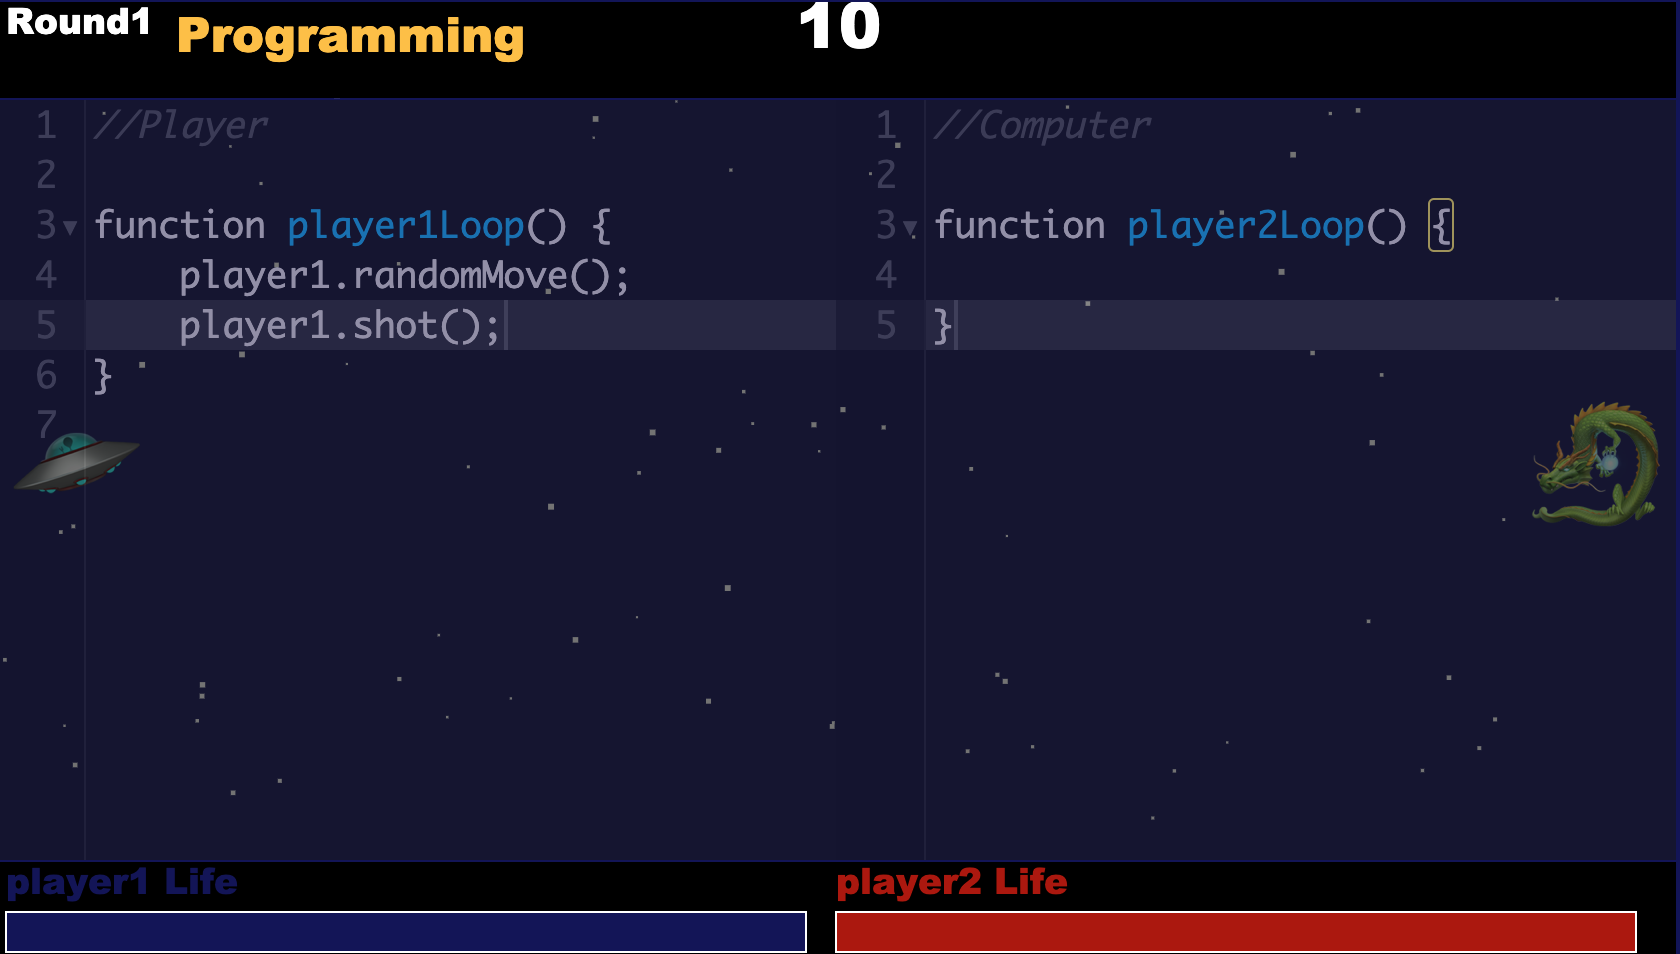
\includegraphics[width=0.8\linewidth]{image/actionProgramming.eps}
  \end{center}
    \vspace{-8mm} 
  \caption{行動プログラミングフェイズの様子}
  \label{actionProgramming}
\end{figure}

\subsubsection{ゲームフェイズ}
このフェイズでは行動プログラミングフェイズで記述したプログラムが10秒間ループして実行され,ゲームが進行する.このフェイズの様子を図\ref{game}に示す.このフェイズに移行した段階で,両プレイヤは相手プレイヤが記述したプログラムを閲覧することができる.このフェイズにおいて相手キャラクタを攻撃し,lifeの値を0以下にしたプレイヤの勝利となる.勝敗が決まらない場合はプログラム終了時の各パラメータを引き継いだまま行動プログラミングフェイズに戻り,再度プログラミングしゲームフェイズに移行するという過程を勝敗が決まるまで繰り返す.

また画面の下には擬似的なコンソールを配置しており,プログラムの実行時に発生したエラーが表示されるため,開発者ツールを開かずとエラーを確認できるようになっている.

\begin{figure}[!ht]
  \begin{center}
    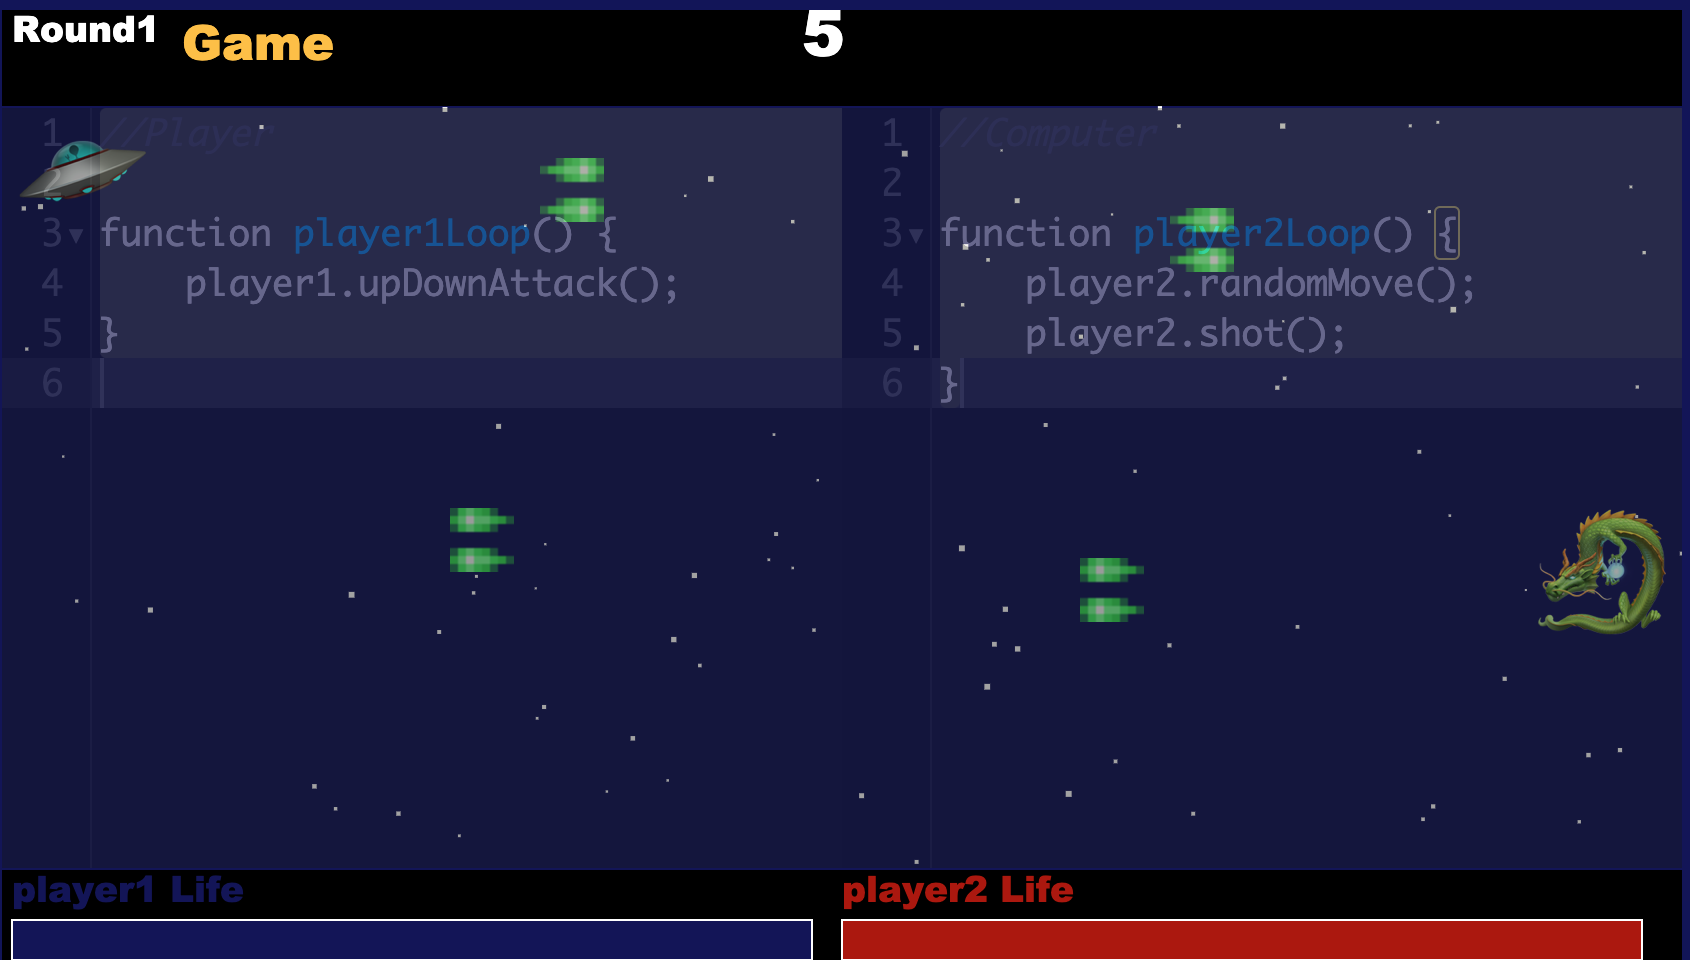
\includegraphics[width=0.8\linewidth]{image/game.eps}
  \end{center}
    \vspace{-8mm} 
  \caption{ゲームフェイズの様子}
  \label{game}
\end{figure}

\subsection{評価実験}
提案システムの使用・観戦に関する感想や影響,その用法を調査するために評価実験を実施した.システムを用いて対戦するプログラマと対戦を観戦するプログラミング初学者を集め,システムでの対戦と観戦を実施し,アンケート調査と実際に対戦で使用されたプログラムのログを分析することでシステムを評価した.

\subsubsection{実験参加者}
実際にゲームをプレイするプログラマとしては,プログラミング(主にオブジェクト指向言語)の経験が3年以上ある大学院生2名(男性)に声をかけた.2名とも日常的にアクションやシューティング等のジャンルのゲームをプレイするため,システムをプレイする際にゲームに不慣れなためハンデが生まれることはないと思われる.また両者とも3年以上JavaScriptを使用した経験がある.

プレイを観戦するプログラミング初学者は,国際人間科学部にて開講されていた講義「プログラミング基礎演習1」の受講者を対象とした.受講者のうち,実験に参加した者は77名であり,うち37名が男性,40名が女性であった.またこの講義ではJavaScriptにおける変数,条件分岐,繰り返しなどの基礎的な文法を教えており,実験参加者は実験を行う時点でこれらを学習済であった.なお,うち23名は授業以前にプログラミングを学習した経験があったが,プログラミングによってソフトウェア開発を行った経験のある者はいなかった.

またプログラマ含む実験参加者の全員が,競技プログラミングやプログラミングゲームなどのプログラミングを題材としたエンタテインメントシステムを使用した経験がなかった.

\subsubsection{実験内容}

初めにプログラマ2人にプログラミングやゲームの経験に関する簡単な事前アンケートを行った後,提案システムにある程度慣れ,用法を理解してもらう必要があるため,システムの練習をするための期間を設けた.システムの使用方法,ゲームシステム,独自に用意したメソッドなどについて説明した後,11/13から11/19の1週間システムを自由に使用させた.また,ただシステムを使用させただけではゲームに対する理解が深まらない可能性があるため,期間中に2つのタスクをこなさせた.1つは1人以上とシステムを使った対人戦を行うことであり,もう1つは相手がランダムな戦略を実行してくる対CPU戦において,勝率が高いと考えられるプログラムを作成することである.

なお期間中はシステムに関する意見・疑問を逐次報告させ,システム使用における問題を改善した.またプログラマがシステムを使用する際に利用するWebブラウザはGoogle Chromeに統一した.

練習期間が終わった翌日に,プログラマ同士の対戦を行った.対戦はシステムに関するプログラマ同士のコミュニケーション等の所作を観察するため,感染症対策を徹底した環境で対面にて行った.両者の対戦時の画面を録画し,対戦後にシステムに関する事後アンケートを行った.なお練習期間中・対戦中にプログラマが記述した全てのコードのログを収集した.

そして「プログラミング基礎演習1」の最終講義で受講者に事前アンケートを行った後,初学者が観戦しやすいように対戦動画を編集したものをzoomを介して閲覧させた.またその後にシステムに関する事後アンケートを行った.

\subsubsection{アンケート結果}

対戦を観戦したプログラミング初学者に対する事後アンケートの内容及び結果を表\ref{interview}に示す.このアンケートに回答したのは実験参加者のうち74名であった.

\begin{table}[H]
  \begin{center}
    \caption{初学者に対する事後アンケート結果}
    \label{beginner_interview}
      \begin{tabular}{|c|c|c|c|c|c|c|c|} \hline
        \multirow{2}{*}{Q} & \multirow{2}{*}{質問項目} & \multicolumn{5}{c}{評価分布} & \multirow{2}{*}{平均} \\
        & & 1 & 2 & 3 & 4 & 5 & \\ \hline\hline
        Q1 & ゲームを観戦するのは楽しかったか & 3 & 6 & 33 & 27 & 5 & 3.34\\ \hline
        Q2 &
        \begin{tabular}{c}
          ゲームの出力はプログラムを理解する\\助けになったか
        \end{tabular}
        & 0 & 9 & 25 & 30 & 10 & 3.55\\ \hline
        Q3 &
        \begin{tabular}{c}
          観戦によってプログラミングに対する\\興味関心は高まったか
        \end{tabular}
        & 1 & 11 & 23 & 33 & 6 & 3.43\\ \hline
        Q4 &
        \begin{tabular}{c}
          観戦によってプログラミングに関する\\理解が深まったか
        \end{tabular}
        & 1 & 23 & 29 & 17 & 4 & 3.00\\ \hline
      \end{tabular}
      \\(1:全くそう思わない, 5:とてもそう思う)
  \end{center}
\end{table}

まずゲーム観戦の楽しさに関して(Q1)であるが,実験参加者の多くが肯定的な回答を示した.またキャラクタが攻撃,移動するなどのゲームの出力がプログラム理解の助けになったかという質問(Q2)に関しても3以上の評価が多かった.さらに観戦によりプログラミングに対する興味関心が高まったかという質問(Q3)についても,3以上の回答が多くなった.また観戦によってプログラミングに関する理解が深まったかという質問(Q4)に関しては,やや低い評価が多い結果となった.なおこれら意外にも以下の質問をした.

\begin{itemize}
  \item Q5.このゲームを実際にプレイしたいか(プレイしたい/プレイしたくない)
  \item Q6.このゲームに他にどのような機能が欲しいか
  \item Q7.このゲームに関する意見
\end{itemize}

まずこのゲームを実際にプレイしたいかという質問(Q5)に関しては64.9\%がプレイしたいと回答した.またこのゲームに他にどのような機能が欲しいかという質問(Q6)に関しては「色んな技が繰り出せるような機能」「通常攻撃以外にため技のようなものが欲しいと思った」「回復アイテム的なものや必殺技」「攻撃を受けたときの衝撃波」などの回答があり,キャラクタの行動,エフェクト,アイテムの概念の追加などを求める意見が多く見られた.また「プログラム内容を解説する機能が欲しい」という意見も複数あり,Q4の結果にも見られるように,プログラムの内容をより分かりやすくする工夫が必要だと考えられる.なおこのゲームに関する意見(Q7)としては,「自分のプログラミングのレベルを上げたいと思った」「面白い」「プログラミングを楽しみながら学習できると言う点でとても面白いと感じた」などゲームに対する肯定的な意見が多く得られた.

しかし「プログラミング初心者には少し難しかった」「楽しめるようになるまでのハードルが高そうだった」「今持っている知識では自分では動かすことが出来ないと感じた」など現状の自分のプログラミングスキルではゲームをプレイするのは難しそうに感じる反応も多く得られた.

またシステムをプレイしたプログラマにも同様に事後アンケートを行った.その内容・結果を表\ref{programmer_interview}に示す.

\begin{table}[!ht]
  \centering
  \caption{プログラマに対する事後アンケート結果}
  \label{programmer_interview}
    \begin{tabular}{|c|c|c|c|} \hline
      \multirow{2}{*}{Q} & \multirow{2}{*}{質問項目} & \multicolumn{2}{c}{プログラマ} \\ 
        & &A&B\\ \hline\hline
      Q1 & システムをプレイするのは楽しかったか & 4 & 5 \\ \hline
      Q2 & ゲームの出力はプログラムを理解する助けになったか & 4 & 5\\ \hline
      Q3 & プレイすることでプログラミングに対する興味関心は高まったか & 3 & 5\\ \hline
      Q4 & プレイによってプログラミングに関する理解が深まったか & 1 & 3\\ \hline
    \end{tabular}
    \\(1:全くそう思わない, 5:とてもそう思う)
\end{table}
この結果についても初学者に対する事後アンケートと同様の傾向があり,Q1,Q2,Q3については肯定的な評価が得られたが,Q4に関しては相対的に評価が低かった.またそれら以外にも以下の質問をした.

\begin{itemize}
  \item Q5.累計何時間程度システムを使用したか
  \item Q6.ゲームの難易度は自分にとって適切だったか
  \item Q7.どのような点が簡単(難しい)と感じたか
  \item Q8.ゲームに他にどのような機能が欲しいか
  \item Q9.今後もこのゲームを使用したいか
  \item Q10.ゲームに関する意見
\end{itemize}

累計何時間程度システムを使用したかという質問(Q5)に関しては1名が2時間,1名が6時間と回答した.またゲームの難易度は自分にとって適切だったかという質問(Q6)に関しては1名が適切だった,1名がやや難しかったと答えた.具体的には(Q7)「リファレンスが乏しくプログラムを書きづら買った」「現状のシステムではある程度システムを使い込んだ人をを想定した作戦を立てづらかった」と回答した.ゲームに他にどのような機能が欲しいかという質問(Q8)に対しては,「オブジェクトが持っている値を確認できるリファレンスのようなものが欲しい」「横移動ができれば,被弾しやすいリスクと引き換えに,敵が来そうな位置で敵より先に弾を打ち込めるチャンスが増える」と回答していた.また今後もこのゲームを使用したいか(Q9)という質問には2名とも「使用したい」と回答した.なおゲームに関する意見は「相手のコードを読んで対処するという部分をもっと積極的にするべきだったかもしれない.ただし,相手の位置に近づくようにプログラムすれば確実に自分が先に被弾するので,自分は動かずに相手が近づくのを待つプログラム以外最良の手がないようにも思う.」というものが得られた.

\subsubsection{コードログ分析結果}

練習期間中・対戦中にプログラマが記述したプログラムのログ,提出したプログラムを分析することで,システムがどのように利用されているか,どのようなプログラムが記述されているかを調査した.分析手法としては各プログラムをパースし,プログラム中のキーワードを抽出した.パーサにはJavaScriptパーサのデファクトスタンダードであるEspria\cite{esprima}を用いた.また各プログラムの可読性についても分析した.その指標としてMcCabeの循環的複雑度\cite{complexity}とSLOC(source lines of code)を用いた.循環的複雑度とはソフトウェア開発におけるソフトウェア測定法であり,プログラム中の分岐の数からプログラムの複雑さを算出する.SLOCはソースコードの行数を意味し,今回は空行やコメント行などを除いた値である論理LOCを用いた.またこれらのパラメータの算出にはJavaScript抽象構文木のソフトウェア複雑性分析ツールであるescomplex\cite{escomplex}を使用した.

\vspace{10truept}
\noindent
{\bf 対CPU戦におけるプログラム分析}

まずvsComputerモードで使用されたプログラムの分析結果について述べる.このモードで使用されたコードは合計327件である.全てのプログラムに含まれていたキーワード(演算子を除く)の個数をグラフ化したものを図\ref{vsComputer_keyword}に示す.

\begin{figure}[H]
  \begin{center}
    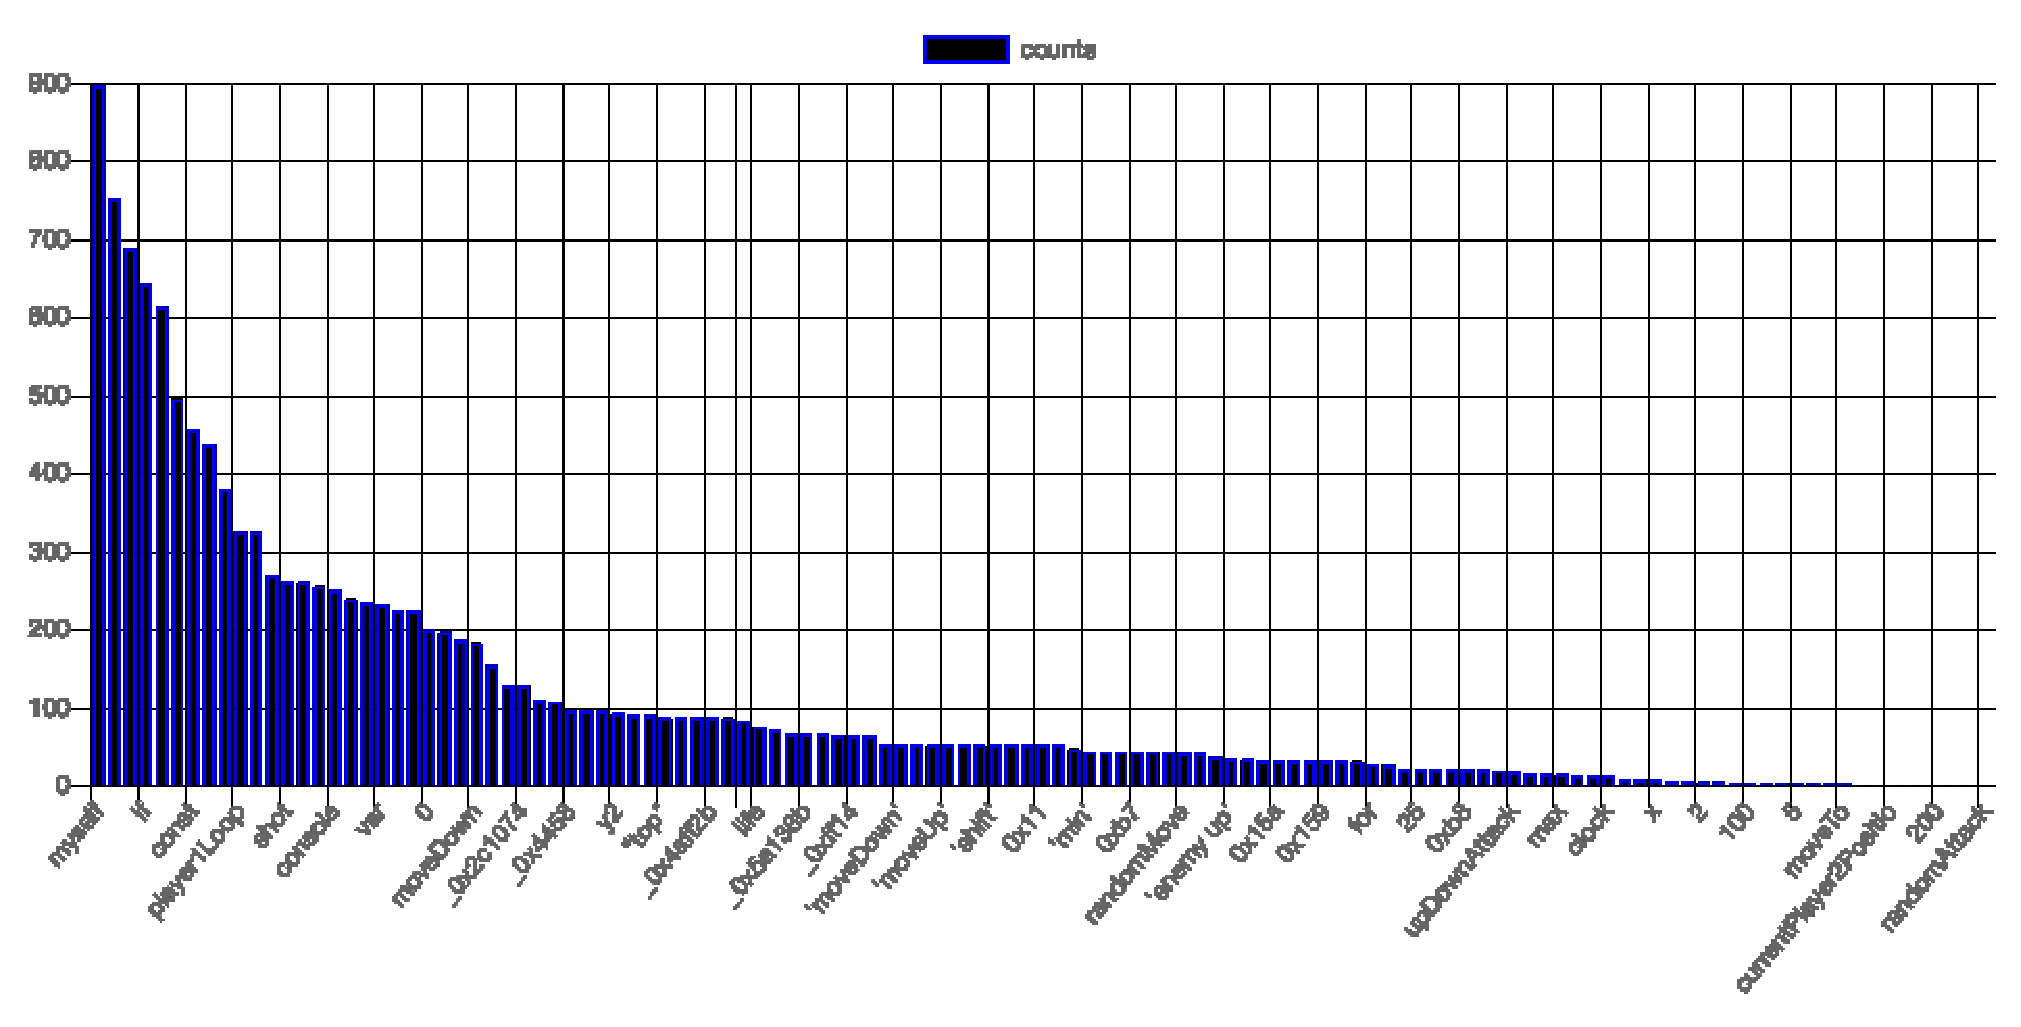
\includegraphics[width=0.9\linewidth]{image/vsComputer_result.eps}
  \end{center}
    \vspace{-8mm} 
  \caption{vsComputerにおけるキーワード分析}
  \label{vsComputer_keyword}
\end{figure}

もっとも多いキーワードはmyselfというものであるがこれは自キャラクタのインスタンスを代入するための変数として使われていた.プロトタイプシステムではプレイヤがplayer1になるかplayer2になるかがランダムに決定されていたため,それによってプログラムの内容を書き換えなくて済むように初めにmyselfに割り当てられたインスタンスを代入していたと思われる.次にplayer1というインスタンスを参照するキーワードが多く見られ,次いでインスタンスの座標を参照するキーワードであるy,条件分岐に用いられるifのキーワードが多く見られた.

プログラムの内容を観察するとキャラクタの座標を参照し,その値によって処理を分岐するプログラムが多く見られ,キーワードの分析結果と一致した.また「0x」で始まるキーワードがいくつか散見されるが,これはプレイヤが難読化ツールを用いてプログラムの難読化を試みた際に現れたキーワードである.


次にvsComputerモードで投稿された各プログラムとSLOC・パラメータ数をグラフ化したものを図\ref{vsComputer_sloc_and_params}表示する.全体として徐々にSLOCが増加する傾向にあり,ゲームに習熟するほどコードの量が長くなっていったのだと考えられるが,無尽蔵にコードの量が増えていく傾向は見られなかった.しかし最大で30行前後のプログラムを初学者が短い時間で読解できるかは議論の余地がある.

またSLOCが平行線をたどり,パラメータの数が増加している部分はプレイヤが難読化ツールを使用した部分である.


\begin{figure}[!b]
  \begin{center}
    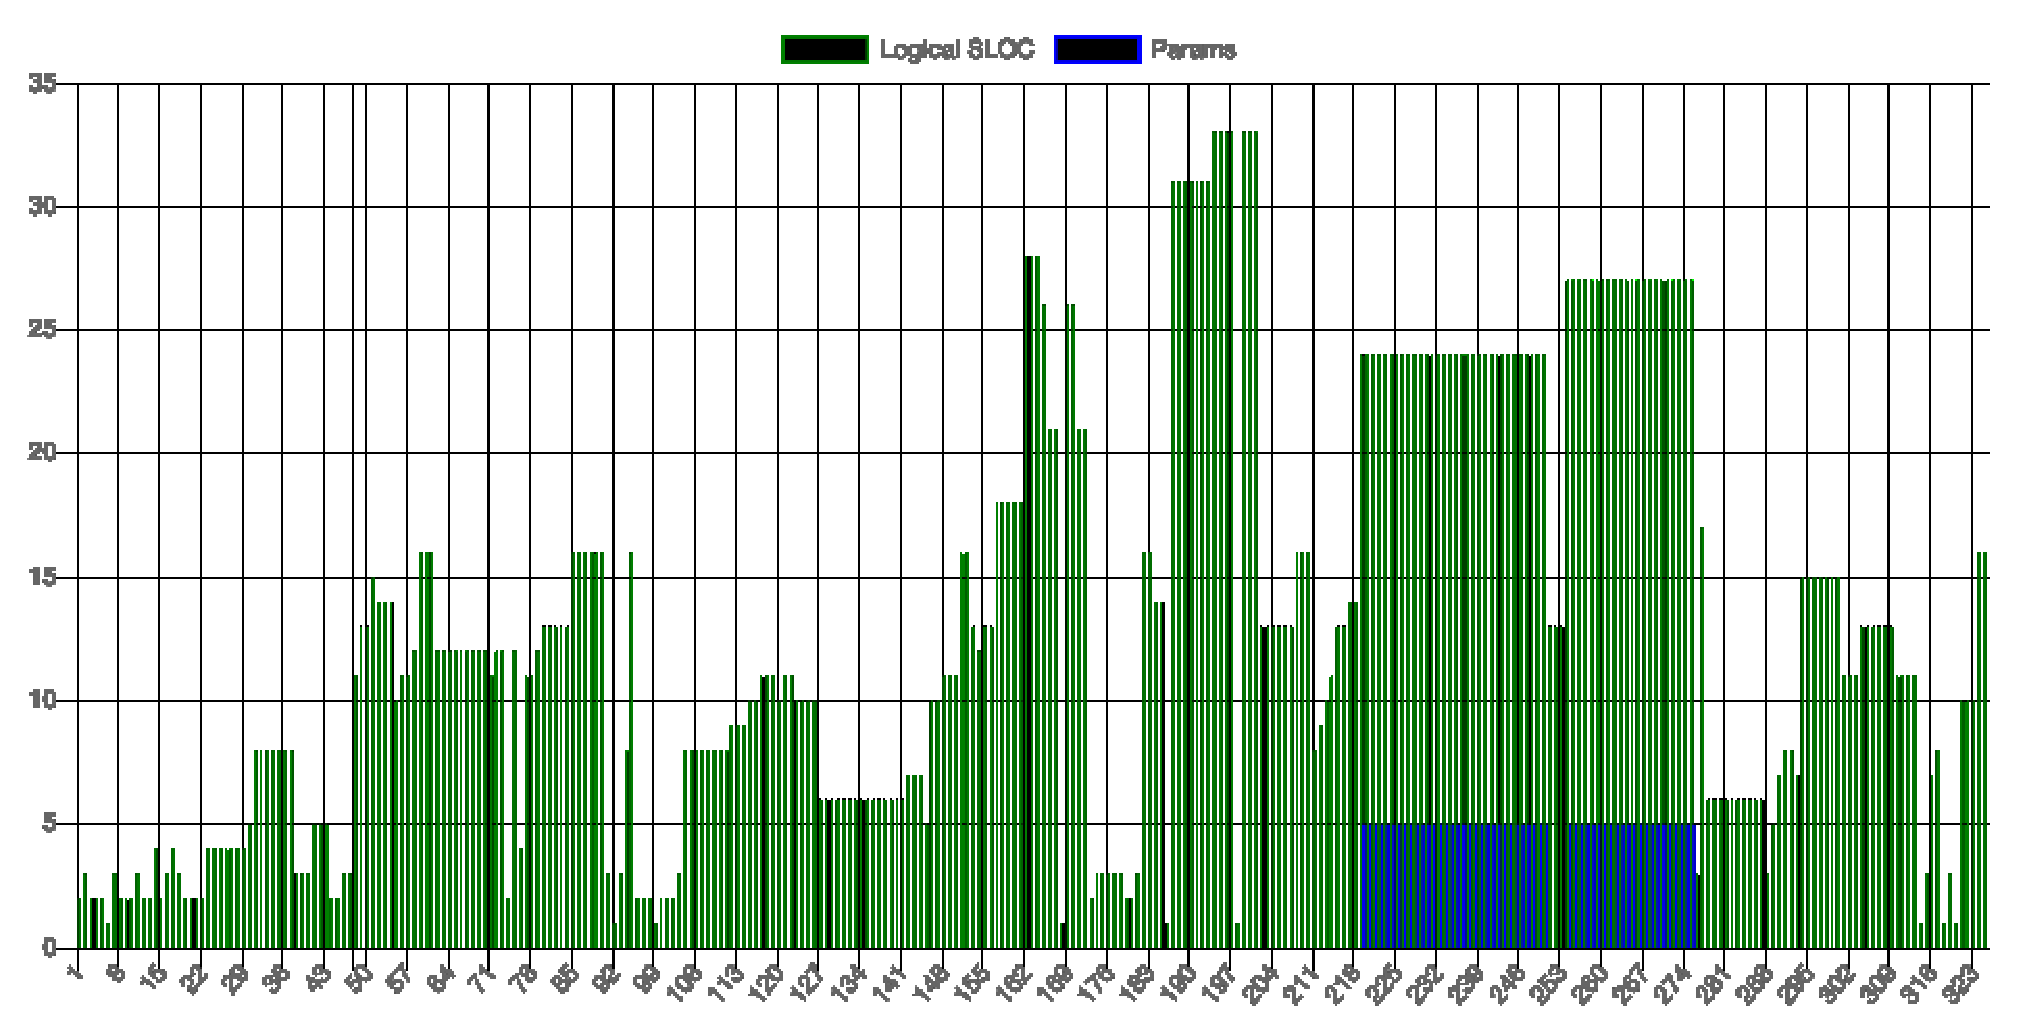
\includegraphics[width=0.9\linewidth]{image/vsComputer_escomplex_SLOC_params.eps}
  \end{center}
    \vspace{-8mm} 
  \caption{vsComputerにおけるSLOCとパラメータ数}
  \label{vsComputer_sloc_and_params}
\end{figure}

次にvsComputerモードにおける各プログラムごとの循環的複雑度を計測したグラフを図\ref{vsComputer_cyclomatic_complexity}示す.このグラフを観察すると各プログラムの循環的複雑度は概ね10以下に収まっていた.McCabeによると循環的複雑度が10を超えるプログラムはモジュール化などの工夫が必要であると述べられているため,今回分析したプログラムは分岐によりプログラムの可読性を大きく損なっていることはないと考えられるが,プログラムを実行する際に循環的複雑度が大きいと実行できないといったような制限を設け,プログラムの可読性が下がらないようにする工夫を設けても良いかもしれない.

\begin{figure}[!h]
  \begin{center}
    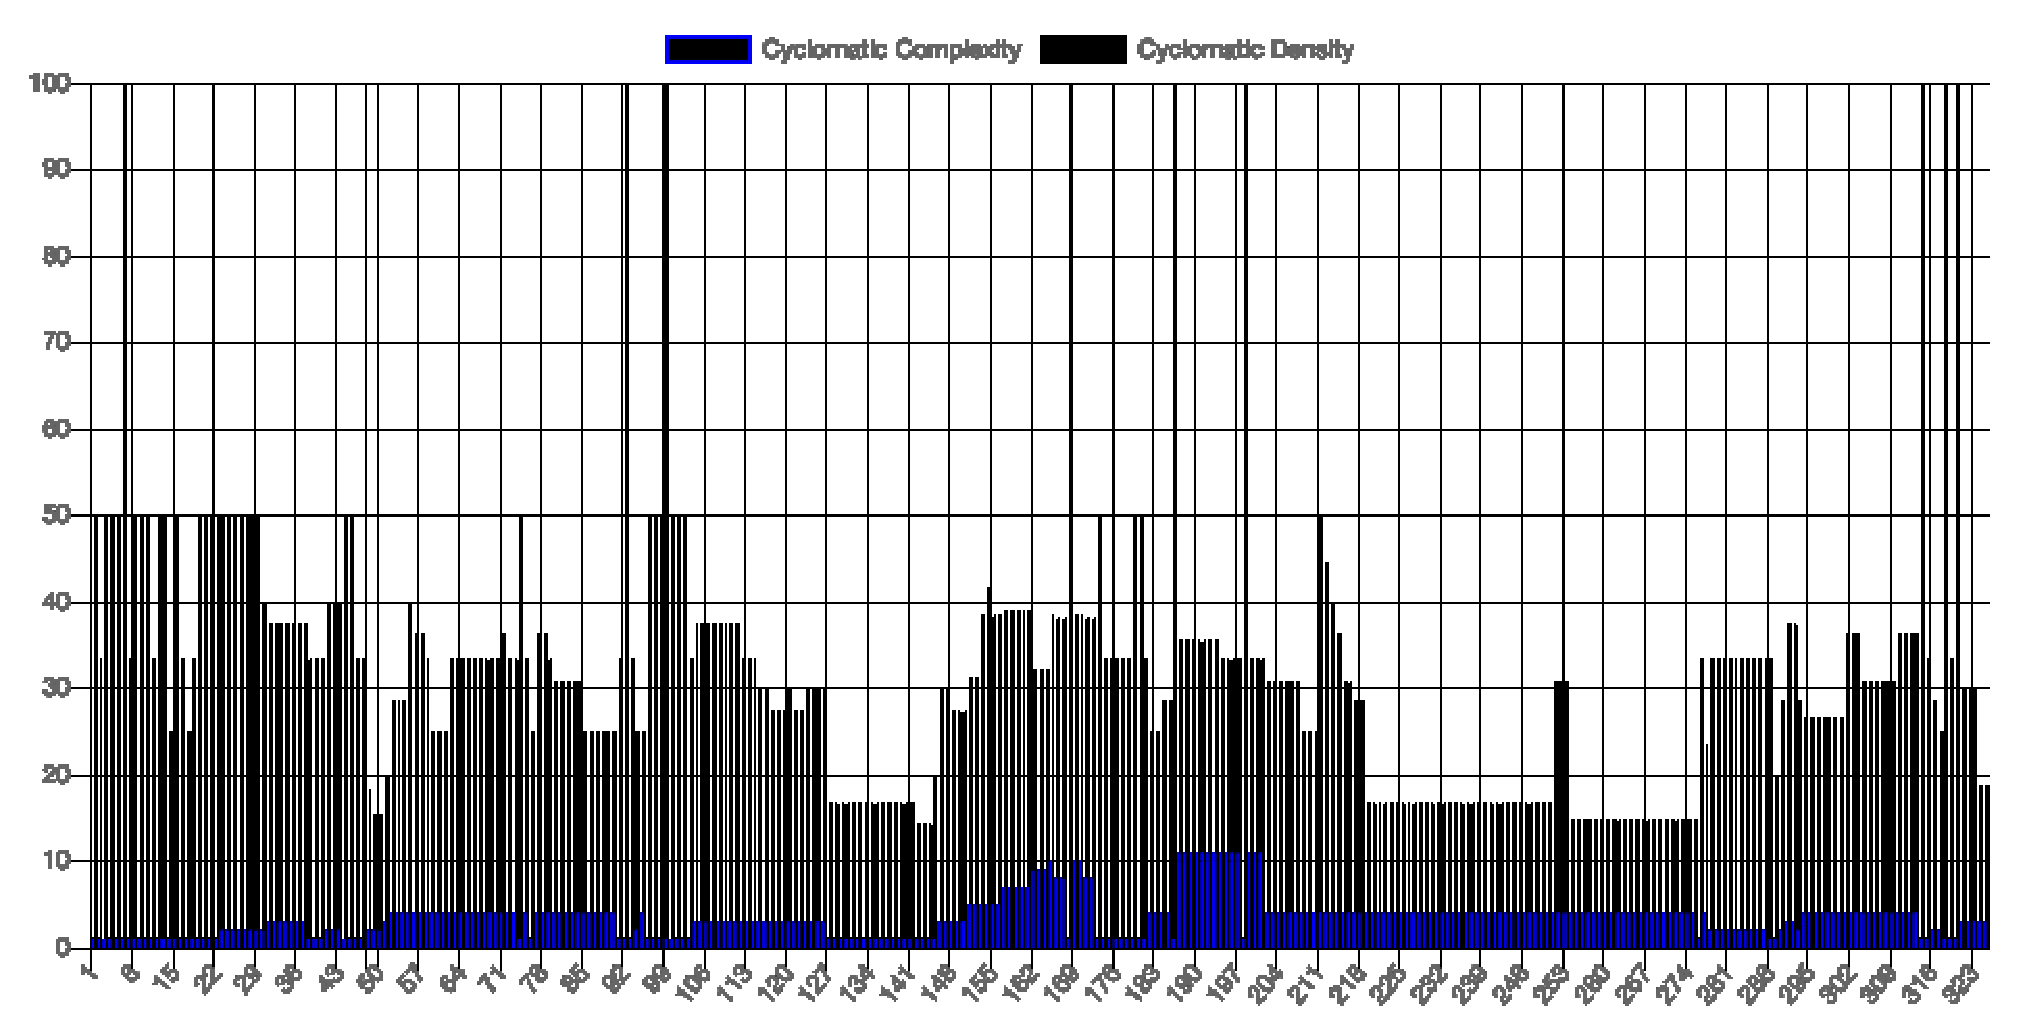
\includegraphics[width=0.9\linewidth]{image/vsComputer_escomplex_complexity.eps}
  \end{center}
    \vspace{-8mm} 
  \caption{vsComputerにおける循環的複雑度とその密度}
  \label{vsComputer_cyclomatic_complexity}
\end{figure}

{\bf 対人戦におけるプログラム分析}

次にvsPlayerモード(対人戦)において使用されたプログラムの分析結果について述べる.このモードで使用されたコードは合計185件である.

全てのプログラムに含まれていたキーワード(演算子を除く)の個数をグラフ化したものを図\ref{vsPlayer_keyword}に示す.

\begin{figure}[H]
  \begin{center}
    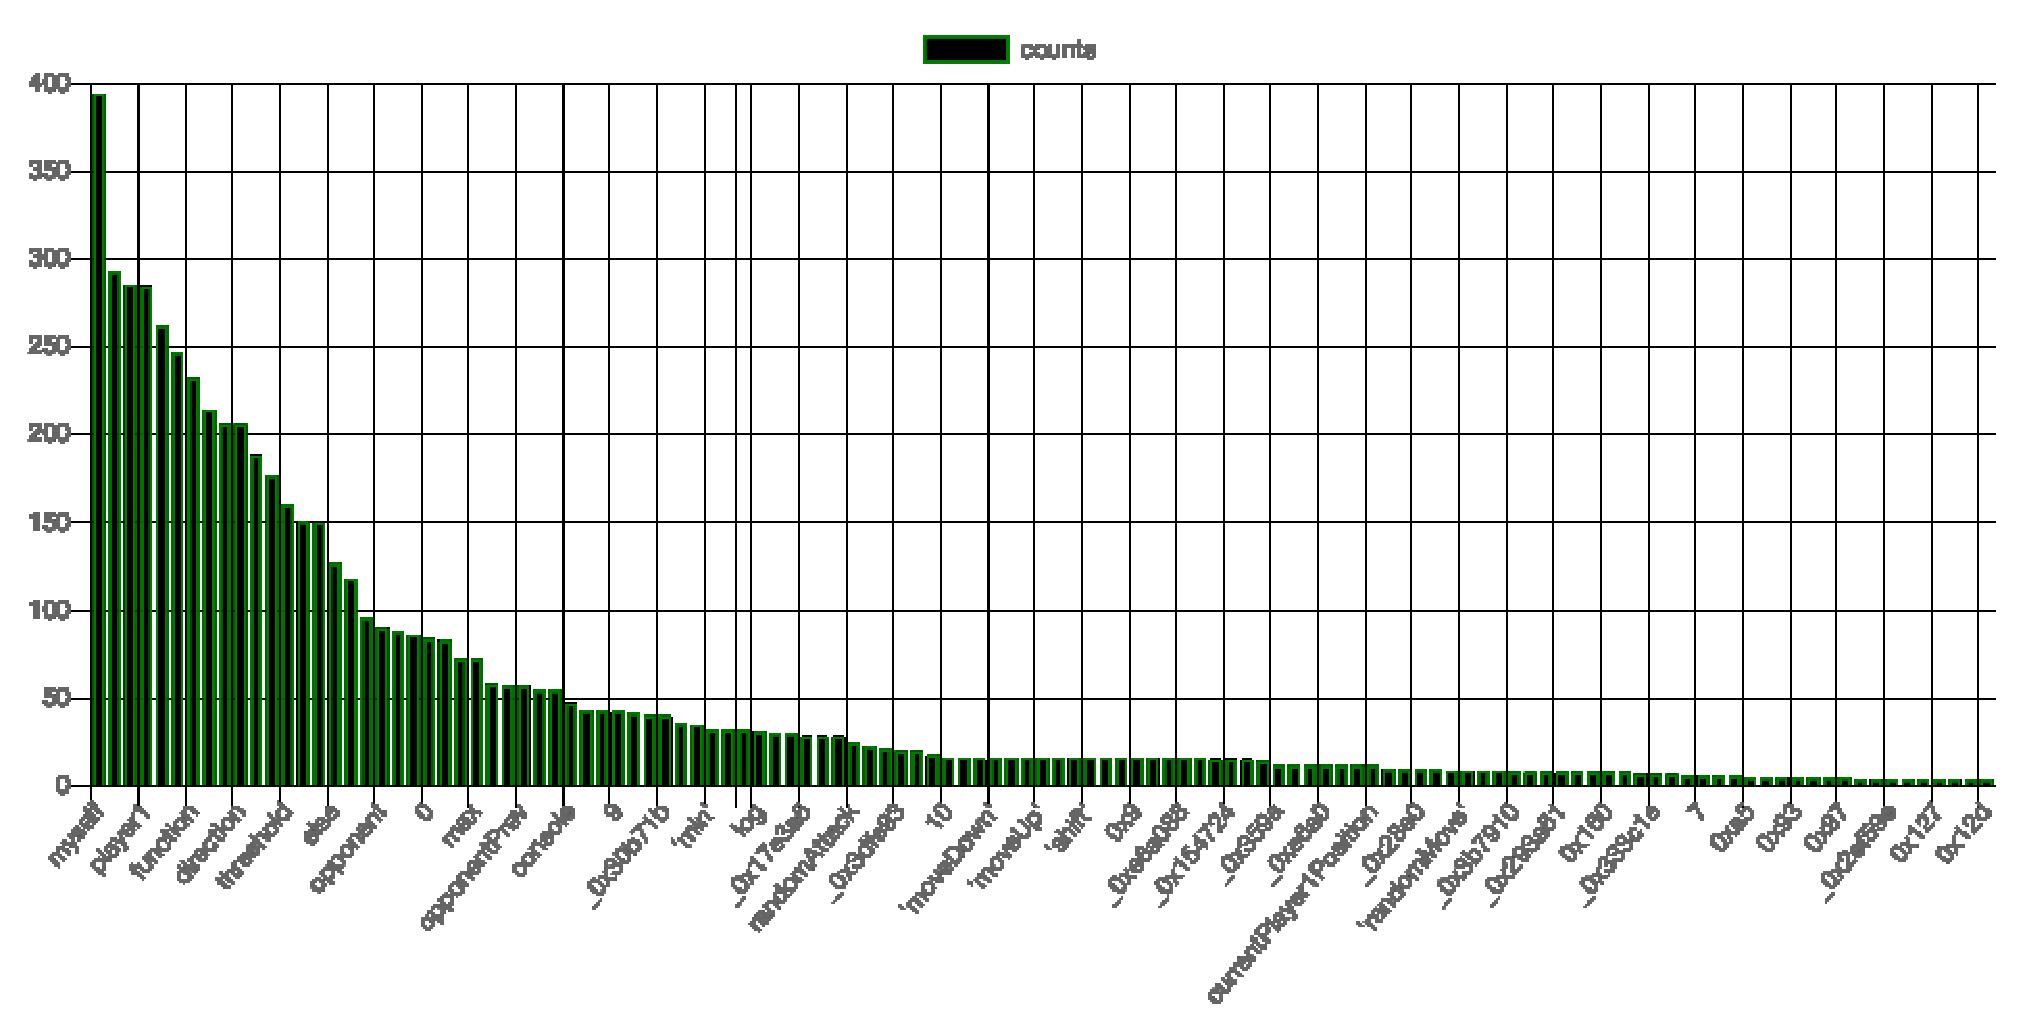
\includegraphics[width=0.9\linewidth]{image/vsPlayer_result.eps}
  \end{center}
    \vspace{-8mm} 
  \caption{vsPlayerにおけるキーワード分析}
  \label{vsPlayer_keyword}
\end{figure}

vsPlayerモードにおいて多かったキーワードは上からmyself,if,yであり,vsComputerモードと同様の傾向が見られた.プログラムの内容もvsComputerモードでのプログラムと大きく変わっておらず,対人戦で使用するプログラムをvsComputerモードで試していたと考えられる.

また各プログラムとSLOC・パラメータ数をグラフ化したものを図\ref{vsPlayer_sloc_and_params}表示する.

\begin{figure}[!b]
  \begin{center}
    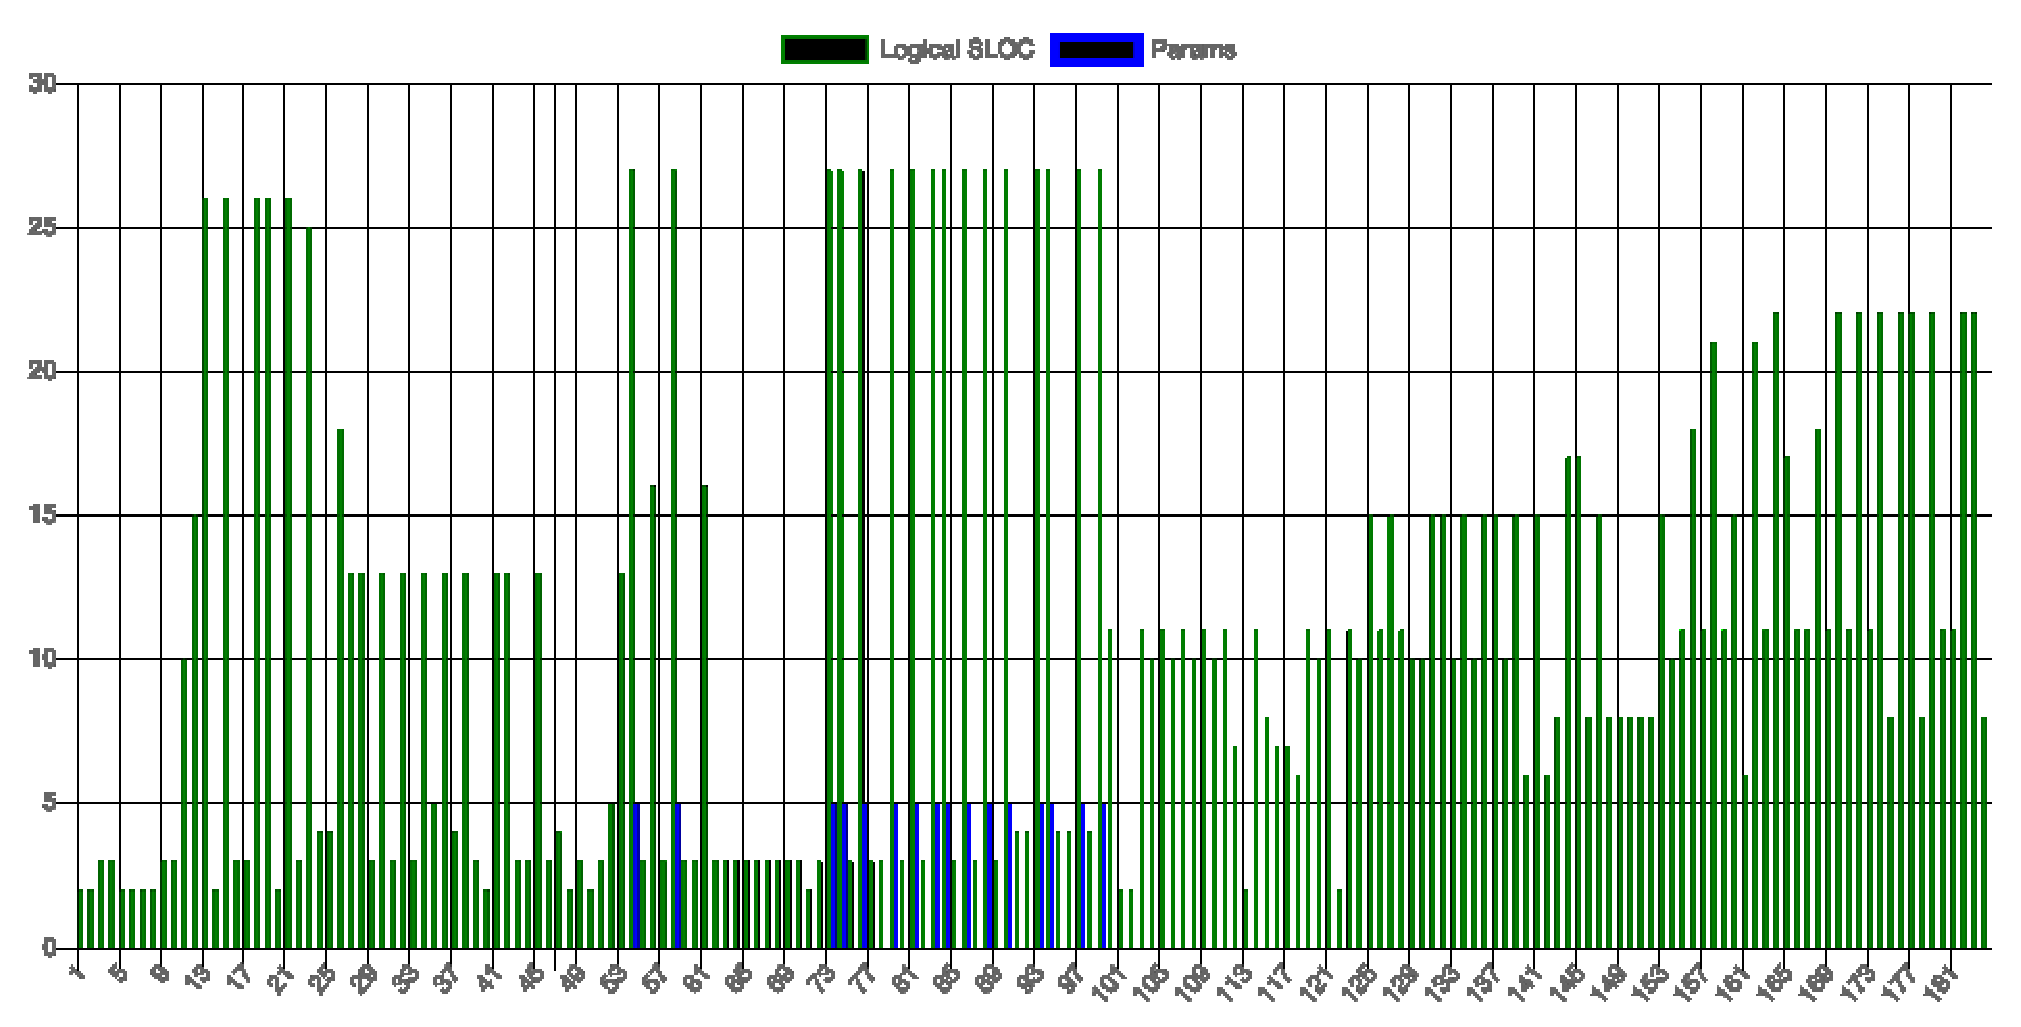
\includegraphics[width=0.9\linewidth]{image/vsPlayer_escomplex_SLOC_params.eps}
  \end{center}
    \vspace{-8mm} 
  \caption{vsPlayerにおけるSLOCとパラメータ数}
  \label{vsPlayer_sloc_and_params}
\end{figure}

次にvsPlayerにおける各プログラムの循環的複雑度を計測したグラフを図\ref{vsPlayer_complexity}示す.vsPlayerにおいても循環的複雑度の最大値は11であり,複雑な分岐はプログラム内に見られなかった.

\begin{figure}[!h]
  \begin{center}
    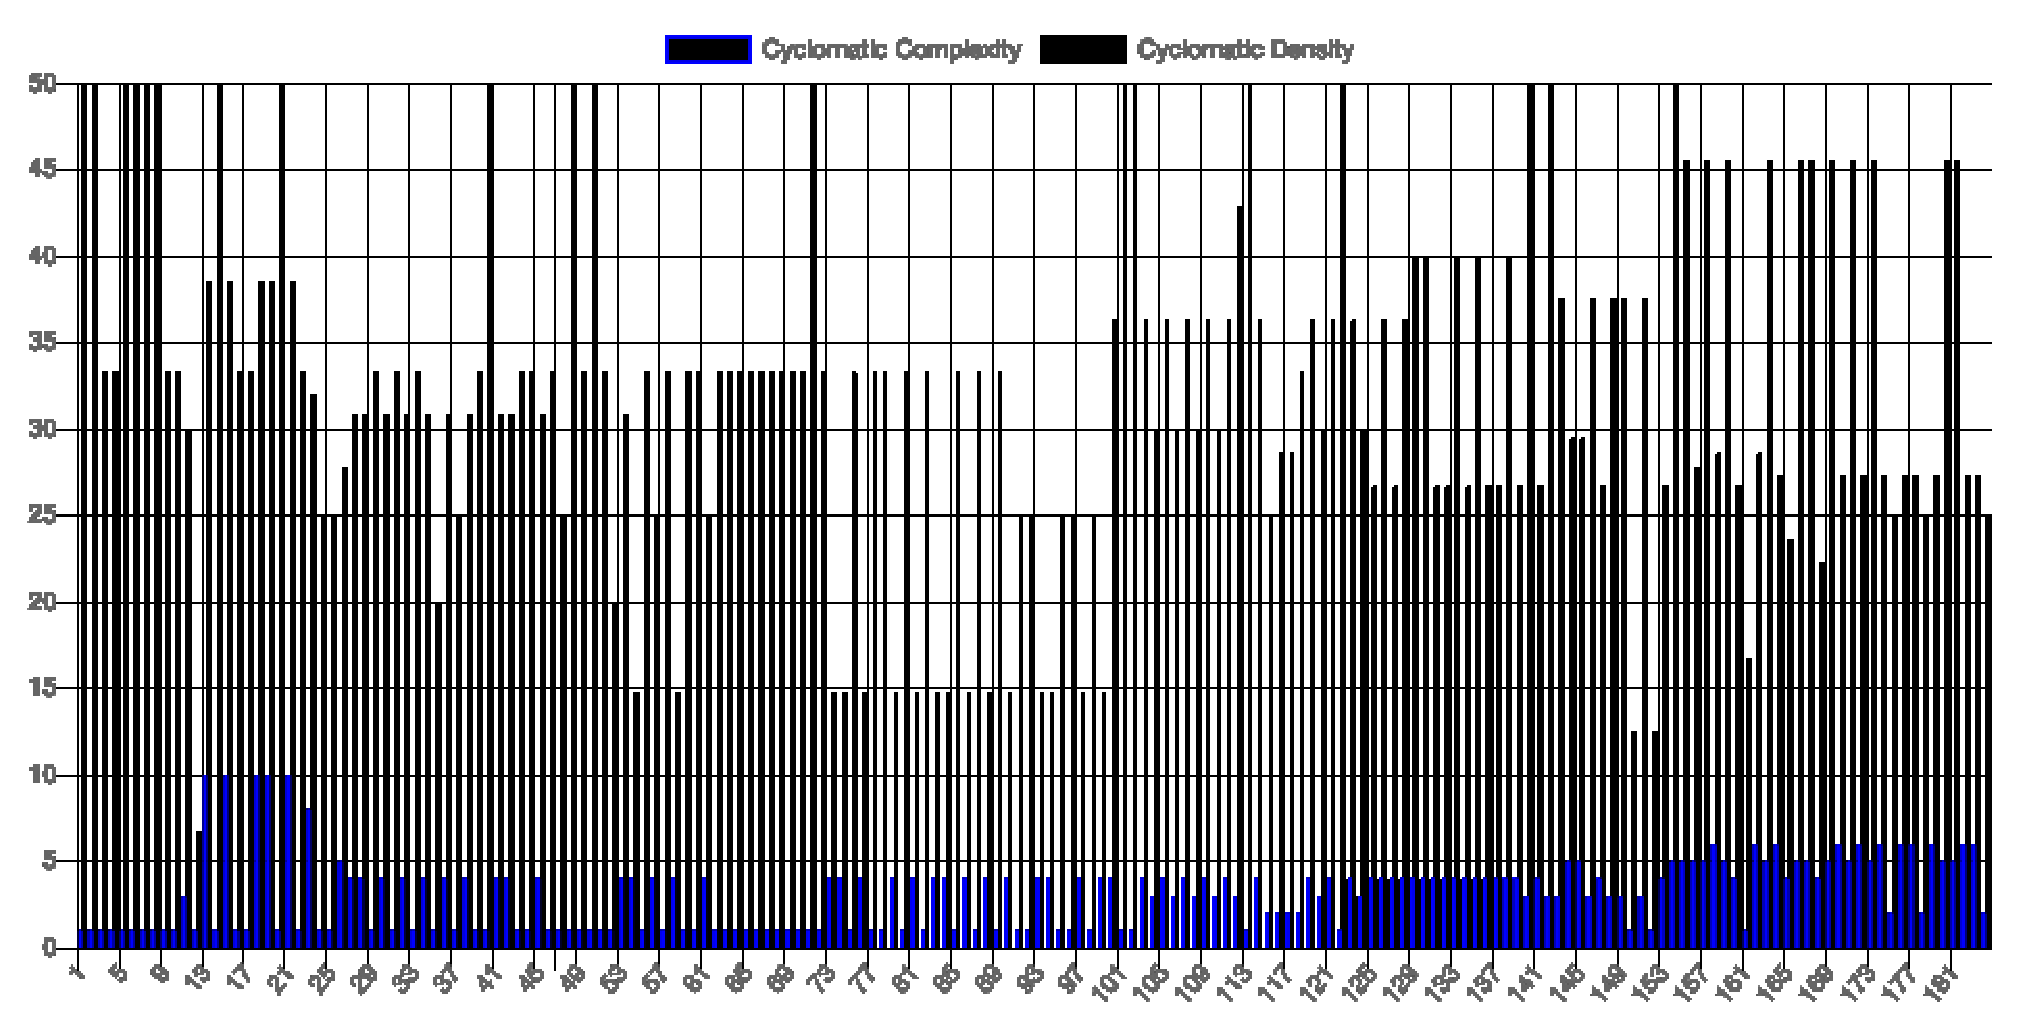
\includegraphics[width=1.0\linewidth]{image/vsPlayer_escomplex_complexity.eps}
  \end{center}
    \vspace{-8mm} 
  \caption{vsPlayerにおける循環的複雑度}
  \label{vsPlayer_complexity}
\end{figure}

\vspace{10truept}
\noindent
{\bf 提出プログラムの分析}

実験に参加したプログラマが提出したコードをソースコード\ref{mishima},\ref{shimizu}に示す.

\begin{lstlisting}[caption=プログラマA, label=mishima]
  const opponent = player1;
  const me = player2;
  let currentPlayer2Position = 240;
  let currentMyPosition = 240;
  function player1Loop() {
      if (currentPlayer2Position === currentMyPosition){
          currentMyPosition - 30 < 0 ? player1.moveDown() : player1.moveUp();
          player1.shot();
      } else {
          currentMyPosition < currentPlayer2Position ? player1.moveDown() : player1.moveUp();
          player1.shot();
      }
      
      currentPlayer2Position = player2.y;
      currentMyPosition = player1.y;
  }
\end{lstlisting}

プログラマAの記述したプログラムは,相手キャラクタと自キャラクタの位置関係によって処理を分岐している.大まかな戦略としては,相手キャラクタと自キャラクタの座標を比較し,同じ位置にいれば上あるいは下に動いて攻撃し,違う位置にいれば相手キャラクタのいる方向へ移動し攻撃する,というものである.

\begin{lstlisting}[caption=プログラマB, label=shimizu]
  const threshold = { min: -17-25, max: 9+25 };
  const myself = player1;
  const enemy = player2;
  function player1Loop() {
      var diff = enemy.y - myself.y;
      var direction = enemy.direction;
      console.log(diff);
      if (diff > threshold.min && diff <= threshold.max) {
          if (direction === "top") {
              myself.moveUp();
          } else if (direction === "bottom") {
              myself.moveDown();
          }
      } else {
          if (diff < threshold.min) {
              myself.moveUp();
          } else if (diff > threshold.max) {
              myself.moveDown();
          }
      }
      myself.shot();
  }
\end{lstlisting}

プログラマBのプログラムもプログラマAと同様,キャラクタの座標を用いた処理を行っているが,キャラクタの向きを表すパラメータであるdirectionも使用している.自キャラクタと相手キャラクタの座標の差分が閾値の範囲内であれば,相手のdirectionを参照して相手と同じ進行方向に移動し攻撃,自キャラクタと相手キャラクタのが大きく異なれば,相手キャラクタから逃げて攻撃するというものである.

初学者が読解するという観点から考えると,これらのプログラムはあまり長くなくネストも深くないため,認知的負荷はそれほど大きくないが数値を用いた条件分岐や三項演算子などは読解する際に慣れが必要なため,やや読解に労力を要すると考えられる.




\subsubsection{評価実験に関する考察}

評価実験に関する考察について述べる.プログラマ同士の対戦においては,行動プログラミングフェイズにおいて設定した相手のappearanceパラメータについて「かわいい」などとコメントする様子が見られた.また対戦後にお互いの記述したプログラムの内容や今までのプログラミング経験等に関するコミュニケーションが行われており,システムがコミュニケーションのきっかけを作ることができていた.また両者の対戦を観察した結果,プログラマがどういったプログラムを記述するか,どうプログラムを変更するかなどについて悩んでいる時間が多いため,リアルタイムな観戦においては,観戦者が飽きないように解説のような機能を入れたり,プログラミングする時間に制限を設けるなどの工夫が必要であると感じた.なおプログラムの内容や戦略がやや一辺倒になってしまっていたため,1つの強い戦略が生まれてしまわないようにより多様なメソッドや強い戦法にリスクを持たせるなどして,多様な戦略を使わせる工夫をする必要があった.さらにプログラマがプレイの際に開発者ツールのコンソールをしている様子が見られ,観戦する際にコンソールを使用している様子はやや初学者にとって内容が分かりづらくなるため,よりシステム画面上のコンソールの機能を拡充し,開発者ツールを使用せずとも対戦できるように設計したい.各々の対戦に着目すると,一方のプログラマの書いたプログラムが他方より圧倒的に強い場合は1ターンで決着がついてしまい,ターン性がうまく機能していない場合があったため,パラメータバランスを調整する必要がある.またプログラマの記述したプログラムを見ると,キャラクタの座標を用いた処理の際に数字を用いていたが,実際にプレイをしたことのない観戦者にとっては数字から具体的な座標をイメージするのが難しいため,極力不要な数値を用いずにプログラムできるように設計することが必要であると感じた.プログラムを開示する際により平易なプログラムに書き換えても良いかもしれない.

初学者の対戦の観戦においては,ライブでプログラマ同士が対戦している状況を用意することが困難であったため今回は動画を閲覧するという状況を用意したが,動画を見ただけでは実際に人が対戦しているという感覚が希薄であり,「プログラマがプログラミングしている」場面を見せるためには更なる工夫が必要であると感じた.

また今回の評価実験において,システムに対する肯定的な評価が得られたものの,どのような要素が初学者のプログラミングに対する興味に影響を与えていたのか,特に提案システムにおいて独特な要素であるリアルタイムな駆け引き・アドリブを誘発する要素の影響について調査する必要があると考えられる.

\subsection{課題と今後の研究}
提案システムの開発・評価実験で明確になった情報を元に,今後どういった研究を行っていくかについて述べる.

\subsubsection{プロトタイプシステムを元にした実環境での運用システムの構築}

評価実験でのアンケート結果・コードログの分析結果を鑑みてより良いゲームデザインが必要であると感じた.まずパラメータバランスを調整し,1ターンで終わるなどすぐにゲームが終わって終わないようにする.またプレイヤ同士の対戦において圧倒的に力の差がある場合でも逆転できるような要素を加えることで,プレイヤ・観戦者がより楽しめるようにする.さらにこのゲームにおける強さがプログラマのスキルに比例し,かつ観戦者にとっても可読性の高いプログラムを表示できるよう,最大コード長に制限を設けたり,循環的複雑度の最大値に制限を儲けるなどの工夫を加える.またプロトタイプシステムではエラーを画面にそのまま表示するだけだったが,プレイヤを積極的にデバッグに向かわせる工夫を加える.これらの工夫に伴いUIを設計し直すとともにキャラクタのエフェクトも観戦に適切なものを採用する.なおvsComputerモードでの対戦に,より戦略的なゲームAIを実装する予定である.さらにユーザログインを実装し,ランキング機能やGitHubアカウントを紐付けてプログラマ同士の交流を図るなどの機能も追加していきたい.

これらの改善を施した上で,実環境で運用するシステムを構築し,より多くのプログラマを対象に利用を呼びかける.

\subsubsection{今後の研究}

今後はシステムに改善を咥えながらより多くのユーザを対象としたワークショップ・実験を行う.より多くの習熟したプログラマを対象とした調査だけでなく,初学者にもゲームをプレイさせ,初学者にとっての影響も調査する.プログラミング言語の基礎的な文法の理解を促すチュートリアルを実装し,プログラミング学習コンテンツとしての効果も調査していきたい.またライブでの対戦を初学者に観戦させ,本システムの特徴であるリアルタイム性・アドリブによる影響を重点的に調査する.なおどうすれば観客が内容を理解し,盛り上がることができるのかといったライブコーディングの見せ方についても調査を行う予定である.さらにリアルタイム性・アドリブが興味喚起に良い影響を及ぼしていたのなら,より若い世代に向けての興味喚起も可能かもしれない.ブロックベースでの制御や,ロボットなどフィジカルなものを制御する試みも行いたい.

今回はリアルタイムなシューティングゲームとしてシステムを実装したが,将棋の対戦に見られるようなプレイヤの熟考と解説者の解説を交えたプログラミングゲームも実現可能かもしれない.より幅広いジャンルのシステムを開発することで,プログラミング初学者向けコンテンツの拡充を目指す.


